\documentclass{apmcmthesis}

\usepackage{url}
\usepackage{indentfirst}
\usepackage{amsmath,amssymb}
\usepackage{graphicx}
\usepackage{booktabs}
\usepackage{float}
\usepackage{enumitem}
\usepackage{caption}
\usepackage{hyperref}

%%%%%%%%%%%%填写相关信息%%%%%%%%%%%%%%%%%%%%%%%%%%
\tihao{C}                            %选题
\baominghao{2612345}           %参赛编号
\begin{document}

\pagestyle{frontmatterstyle}

\begin{abstract} 
    
% 论文摘要：
This is abstract of this thesis

% 论文关键词
\keywords{Keywords1\quad  Keywords2\quad   Keywords3}
\end{abstract}



\newpage
%目录
\tableofcontents


\newpage
\pagestyle{mainmatterstyle}
\setcounter{page}{1}

\section{Introduction}

\subsection{this is a subsection of Introduction}
this is the content


\section{Q1}

% ==================================================
% 2.1 中国大豆进口贸易分析
% ==================================================

\subsection{中国大豆进口贸易分析}
\label{subsec:soybean_trade_analysis}

2024年，巴西、美国和阿根廷三国对华大豆出口总量约为
1.035亿吨，出口总额约为459.5亿美元，占中国总大豆进口量的95\%。
从长期变化趋势来看，中国大豆进口来源结构发生了显著变化：
巴西的市场份额持续提升，美国仍是中国大豆进口的重要来源国，
而阿根廷在中国大豆进口市场中的相对地位则有所下降。
总体而言，中国大豆进口来源逐渐形成以巴西为主、美国次之、
阿根廷所占份额相对较低的贸易格局。

\subsubsection{2015--2024年中国大豆进口贸易的变化趋势}

为分析中国大豆进口来源结构的长期演变，本文选取2015年和2024年
作为比较时点，从出口数量、出口金额及其变化幅度等方面，
对巴西、美国和阿根廷三国对华大豆贸易进行比较。
具体结果如表~\ref{tab:soybean_trade_trend}所示。

\begin{table}[H]
    \centering
    \caption{2015年与2024年三国对华大豆出口情况比较}
    \label{tab:soybean_trade_trend}
    \begin{tabular}{lccc}
        \toprule
        指标 & 2015年 & 2024年 & 变化幅度 \\
        \midrule
        三国对华出口总量
        & 7797万吨
        & 1.035亿吨
        & +32.8\% \\

        三国对华出口总额
        & 298.5亿美元
        & 459.5亿美元
        & +53.9\% \\

        巴西对华出口
        & 4093万吨 / 157.9亿美元
        & 7256万吨 / 315.0亿美元
        & +77.3\% / +99.5\% \\

        美国对华出口
        & 2732万吨 / 105.2亿美元
        & 2706万吨 / 127.6亿美元
        & -1.0\% / +21.3\% \\

        阿根廷对华出口
        & 972万吨 / 35.4亿美元
        & 392万吨 / 16.9亿美元
        & -59.7\% / -52.2\% \\
        \bottomrule
    \end{tabular}
\end{table}

\paragraph{巴西：对华大豆出口地位持续提升。}

在研究期内，巴西逐渐成为中国大豆进口的主要来源国。
其对华大豆出口份额由2015年的52.5\%上升至2024年的70.1\%。
2023年，巴西对华大豆出口量达到7447万吨，创下研究期内的历史峰值。
上述变化表明，巴西在中国大豆进口来源结构中的地位不断增强，
中国大豆进口对巴西的依赖程度也随之提高。

\paragraph{美国：贸易摩擦冲击后出口有所恢复，但市场份额尚未完全恢复。}

2018年中美贸易摩擦对美国大豆对华出口产生了显著影响。
美国对华大豆出口量由2017年的3169万吨下降至2018年的824万吨，
其市场份额由34.4\%降至10.3\%。
同期，巴西对华大豆出口份额上升至85.5\%，
反映出贸易政策冲击期间中国大豆进口来源结构发生了显著调整。

2020年中美第一阶段经贸协议签署后，美国对华大豆出口逐步恢复，
出口量回升至约3000万吨的水平。然而，其市场份额仍处于约26\%的水平，
尚未恢复至十年前的相对地位。
这一变化表明，贸易政策冲击可能显著影响大豆进口来源结构，
而贸易关系缓和并不必然意味着原有市场份额能够完全恢复。

\paragraph{阿根廷：对华大豆出口规模总体收缩。}

阿根廷在中国大豆进口市场中的份额总体呈下降趋势。
2015年，其对华大豆出口份额为12.5\%，而2023年已降至1.7\%，
当年出口量仅为174万吨。
这一变化与2022/2023年度阿根廷遭遇严重干旱、
国内大豆产量下降等因素有关。

2024年，阿根廷对华大豆出口量回升至392万吨，
市场份额回升至3.8\%，但仍明显低于2015年的水平。
因此，阿根廷在中国大豆进口来源结构中的相对地位
尚未恢复至研究期初的水平。

\begin{figure}[H]
    \centering
    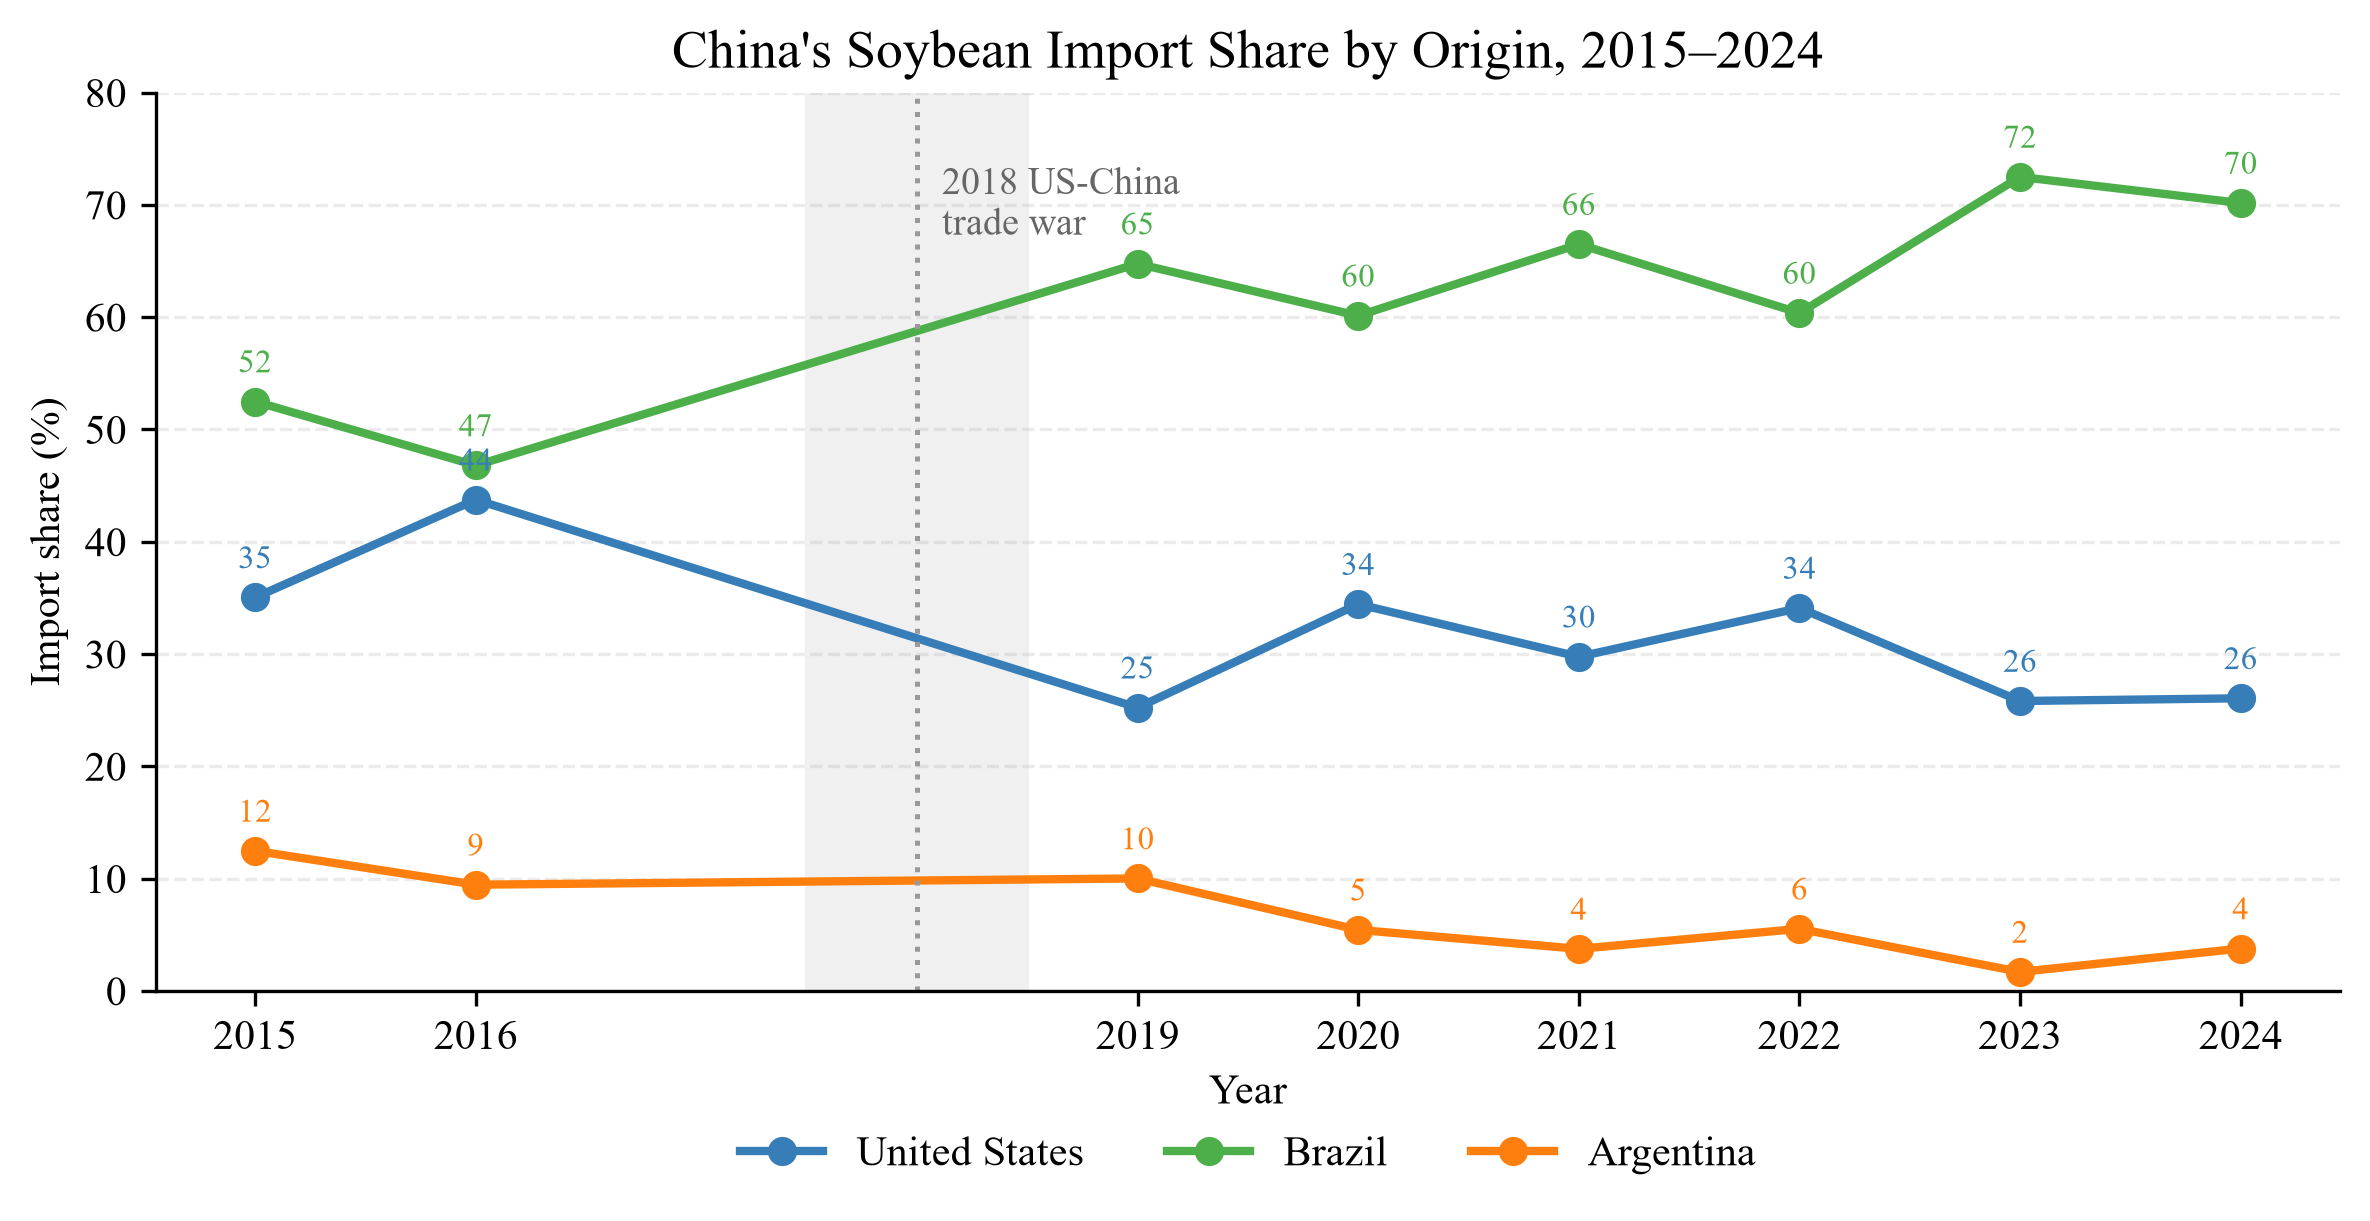
\includegraphics[width=1\textwidth]
    {../images/fig_historical_shares.png}
    \caption{2015--2024年三国对华大豆出口份额变化趋势}
    \label{fig:historical_shares}
\end{figure}

\subsubsection{中国大豆进口价格走势}

除出口数量与贸易份额外，价格变化也是影响大豆进口贸易金额的重要因素。
研究期内，中国进口大豆的平均单价由2015年的383美元/吨
上升至2022年的591美元/吨，随后有所回落，2024年降至444美元/吨。

从整体变化来看，2015年至2024年，三国对华大豆出口总额增长53.9\%，
高于出口总量32.8\%的增幅。
这一差异表明，除进口数量增长外，进口价格变化也对贸易总额增长
产生了重要影响。结合平均进口单价的变化可以看出，
价格因素是研究期内中国大豆进口贸易金额增长的重要组成部分。

\subsubsection{贸易格局变化与后续模型研究的引出}

从图~\ref{fig:historical_shares}可以看出，
2023年和2024年三国对华大豆出口份额的年度变化相对有限，
表明这两年中国大豆进口来源结构总体保持相对稳定。

基于这一现象，本文进一步研究2025年美国相关关税政策变化
对中国大豆进口来源结构可能产生的影响。
在后续模型中，本文将关税政策视为影响2025年三国对华大豆出口份额的
关键因素，并在基准情景下假设其他影响因素保持不变。

% ==================================================
% 2.2 第一问模型的建立与求解
% ==================================================

\subsection{模型的建立与求解}
\label{subsec:model_q1}

2025年，美国宣布调整对华关税政策后，
中国也针对包括美国大豆在内的部分进口产品提出了相应的反制关税措施。
在此背景下，本文借鉴国际贸易理论中常替代弹性
（Constant Elasticity of Substitution, CES）函数的基本思想，
建立中国大豆进口来源份额模型，以预测不同关税情景下，
中国从美国、巴西和阿根廷进口大豆的份额变化。

模型以2024年为基准年，利用基准年实际贸易数据校准相关参数，
并通过设置不同关税情景，分析关税变化对三国进口份额的潜在影响。
此外，本文选取2018年中美贸易摩擦期间的历史贸易数据进行回测，
以检验模型对关税冲击及进口来源结构变化的解释能力。

\subsubsection{模型假设与合理性说明}

为突出关税政策对中国大豆进口来源结构的影响，
并在现有数据条件下建立可求解的数学模型，本文作出以下假设。

\begin{enumerate}[label=\arabic*., leftmargin=2.5em]

    \item \textbf{替代弹性保持不变。}

    本文假设美国、巴西和阿根廷生产的大豆属于不完全替代品。
    尽管三国出口的大豆在用途上具有一定相似性，
    但产地、品质及其他产品特征可能存在差异，
    因此不能将不同来源的大豆视为完全同质的商品。
    本文使用替代弹性参数$\sigma$刻画不同来源大豆之间的替代程度，
    并假设三国之间的替代弹性参数相同，且在预测期间保持不变。

    \item \textbf{进口来源范围保持不变。}

    由于美国、巴西和阿根廷对华大豆出口占中国进口的95\%，本文仅考虑中国从美国、巴西和阿根廷
    进口大豆。因此，三国大豆进口份额之和为1，即
    \begin{equation}
        \sum_{i\in\{\mathrm{US},\mathrm{BR},\mathrm{AR}\}}s_i=1,
        \label{eq:share_sum}
    \end{equation}
    其中，$s_i$表示国家$i$在中国大豆进口总量中的份额，
    $\mathrm{US}$、$\mathrm{BR}$和$\mathrm{AR}$分别代表美国、巴西和阿根廷。

    \item \textbf{出口国基准价格保持不变。}

    本文假设美国、巴西和阿根廷大豆的基准出口价格$p_i$
    在模型预测期间保持不变，不考虑出口国因关税变化而主动调整报价的情形。
    在此假设下，关税变化通过改变进口大豆的含税价格影响中国的进口来源选择，
    进而引起不同国家进口份额的变化。

    \item \textbf{中国大豆进口总需求保持不变。}

    本文假设研究期间中国大豆进口总需求保持不变。
    因此，模型主要用于分析不同来源国之间的进口份额重新分配，
    而不直接预测关税变化引起的中国大豆进口总量变化。

    \item \textbf{其他影响因素通过来源国偏好参数统一表征。}

    考虑到国家产能约束、汇率波动、出口国降价策略及产品质量差异等因素
    均可能影响中国大豆进口来源的选择，
    本文使用来源国偏好参数$\alpha_i$概括这些因素的综合影响，
    并假设该参数在预测情景下保持不变。
    这一处理有助于突出关税变化的相对影响，
    但也意味着模型无法完全反映供给冲击、相对价格调整
    及其他非关税因素所造成的实际变化。

\end{enumerate}

\subsubsection{模型参数的确定}

本文需要确定替代弹性参数$\sigma$、关税参数$\tau_i$
以及来源国偏好参数$\alpha_i$。
其中，$\sigma$用于刻画不同来源大豆之间的替代程度，
$\tau_i$用于描述国家$i$所面临的关税水平，
$\alpha_i$则根据基准年的实际进口份额进行校准。

本文采用以下进口份额公式和出口国到岸价格公式：

\begin{equation}
    s_i =
    \frac{\alpha_i^{\sigma}P_i^{\,1-\sigma}}
    {\displaystyle\sum_j \alpha_j^{\sigma}P_j^{\,1-\sigma}},
    \qquad
    P_i=p_i(1+\tau_i),
    \label{eq:ces_import_share}
\end{equation}

其中，$s_i$表示国家$i$在中国大豆进口总量中的份额，
$\alpha_i$表示国家$i$的来源国偏好参数，
$\sigma$表示来源间替代弹性，
$P_i$表示国家$i$大豆的含税到岸价格，
$p_i$表示其基准出口价格，
$\tau_i$表示模型中定义的关税税率。
分母对所有纳入模型的进口来源国求和。

\paragraph{（1）替代弹性参数$\sigma$的确定}

本文参考GTAP数据库中油籽类商品的来源间替代弹性参数
（ESUBM），其参考值为4.9。
原始研究框架拟将$\sigma=4.0$作为基准情景下的中心参数值，
并将其作为敏感性分析中的一种设定。

\textit{（此处补充GTAP数据库或相关学术文献的规范引用。）}

\paragraph{（2）关税参数$\tau_i$的确定}

为考察不同关税水平对中国大豆进口来源结构的影响，
本文设置以下三种关税情景：

\begin{enumerate}[label=\arabic*., leftmargin=2.5em]

    \item \textbf{低关税情景：$S_{1,\mathrm{low}}=10\%$.}

    该情景对应原始研究框架所采用的3月4日公告中的大豆专项反制税率，
    用于分析较低关税水平下进口来源份额的变化。
    具体政策依据及税率适用范围应以正式政策文件为准。

    \item \textbf{中等关税情景：$S_{2,\mathrm{mid}}=20\%$.}

    该情景对应原始研究框架中日内瓦经贸会谈后所设定的关税水平，
    即由10\%专项关税与保留的10\%对等关税构成。
    该情景用于分析中等关税水平下中国大豆进口来源结构的潜在变化。
    具体税率的生效时间、适用范围及叠加关系应根据正式政策文件核实。

    \item \textbf{高关税情景：$S_{3,\mathrm{high}}=34\%$.}

    该情景对应原始研究框架中4月对等关税政策所采用的名义税率，
    用于考察较高关税冲击下进口来源结构的潜在变化。
    相关税率及其适用范围应在最终论文中补充权威来源。

\end{enumerate}

\textit{（此处补充相关关税政策公告及官方文件的规范引用。）}

\paragraph{（3）来源国偏好参数$\alpha_i$的确定}

本文选取2024年作为基准年，根据该年度美国、巴西和阿根廷对华大豆出口
的实际数据，反推出模型中的来源国偏好参数$\alpha_i$，如下表所示。

\begin{table}[H]
  \centering
  \caption{三国大豆偏好参数 $\alpha_i$ 校准值（$\sigma=4.0$）}
  \label{tab:alpha}
  \begin{tabular}{lccc}
    \toprule
    国家 & 代码 & $\alpha_i$ & 经济含义 \\
    \midrule
    巴西 & BRA & 86.77 & 最高；中国对其``天然偏好''最强（基准份额 70.2\%） \\
    美国 & USA & 72.30 & 次之 \\
    阿根廷 & ARG & 41.76 & 最低（基准份额仅 3.8\%） \\
    \bottomrule
  \end{tabular}
\end{table}

在给定基准年的进口份额、基准出口价格及替代弹性参数的条件下，
通过式~\eqref{eq:ces_import_share}进行参数校准，
使模型能够再现2024年的实际进口来源结构。
校准完成后，将所得偏好参数用于不同关税情景下的份额预测。

需要注意的是，来源国偏好参数的具体数值取决于实际进口份额、
基准出口价格及替代弹性参数的取值。

\subsubsection{模型预测}

在确定来源国偏好参数$\alpha_i$、替代弹性参数$\sigma$
以及不同关税情景下的关税参数$\tau_i$后，
本文利用式~\eqref{eq:ces_import_share}计算2025年不同关税情景下
中国从美国、巴西和阿根廷进口大豆的份额。

模型预测结果通过图~\ref{fig:scenario_qty_value}和
图~\ref{fig:scenario_donut}展示，
分别用于呈现不同关税情景下的预测结果及进口来源份额结构。

\begin{figure}[H]
    \centering
    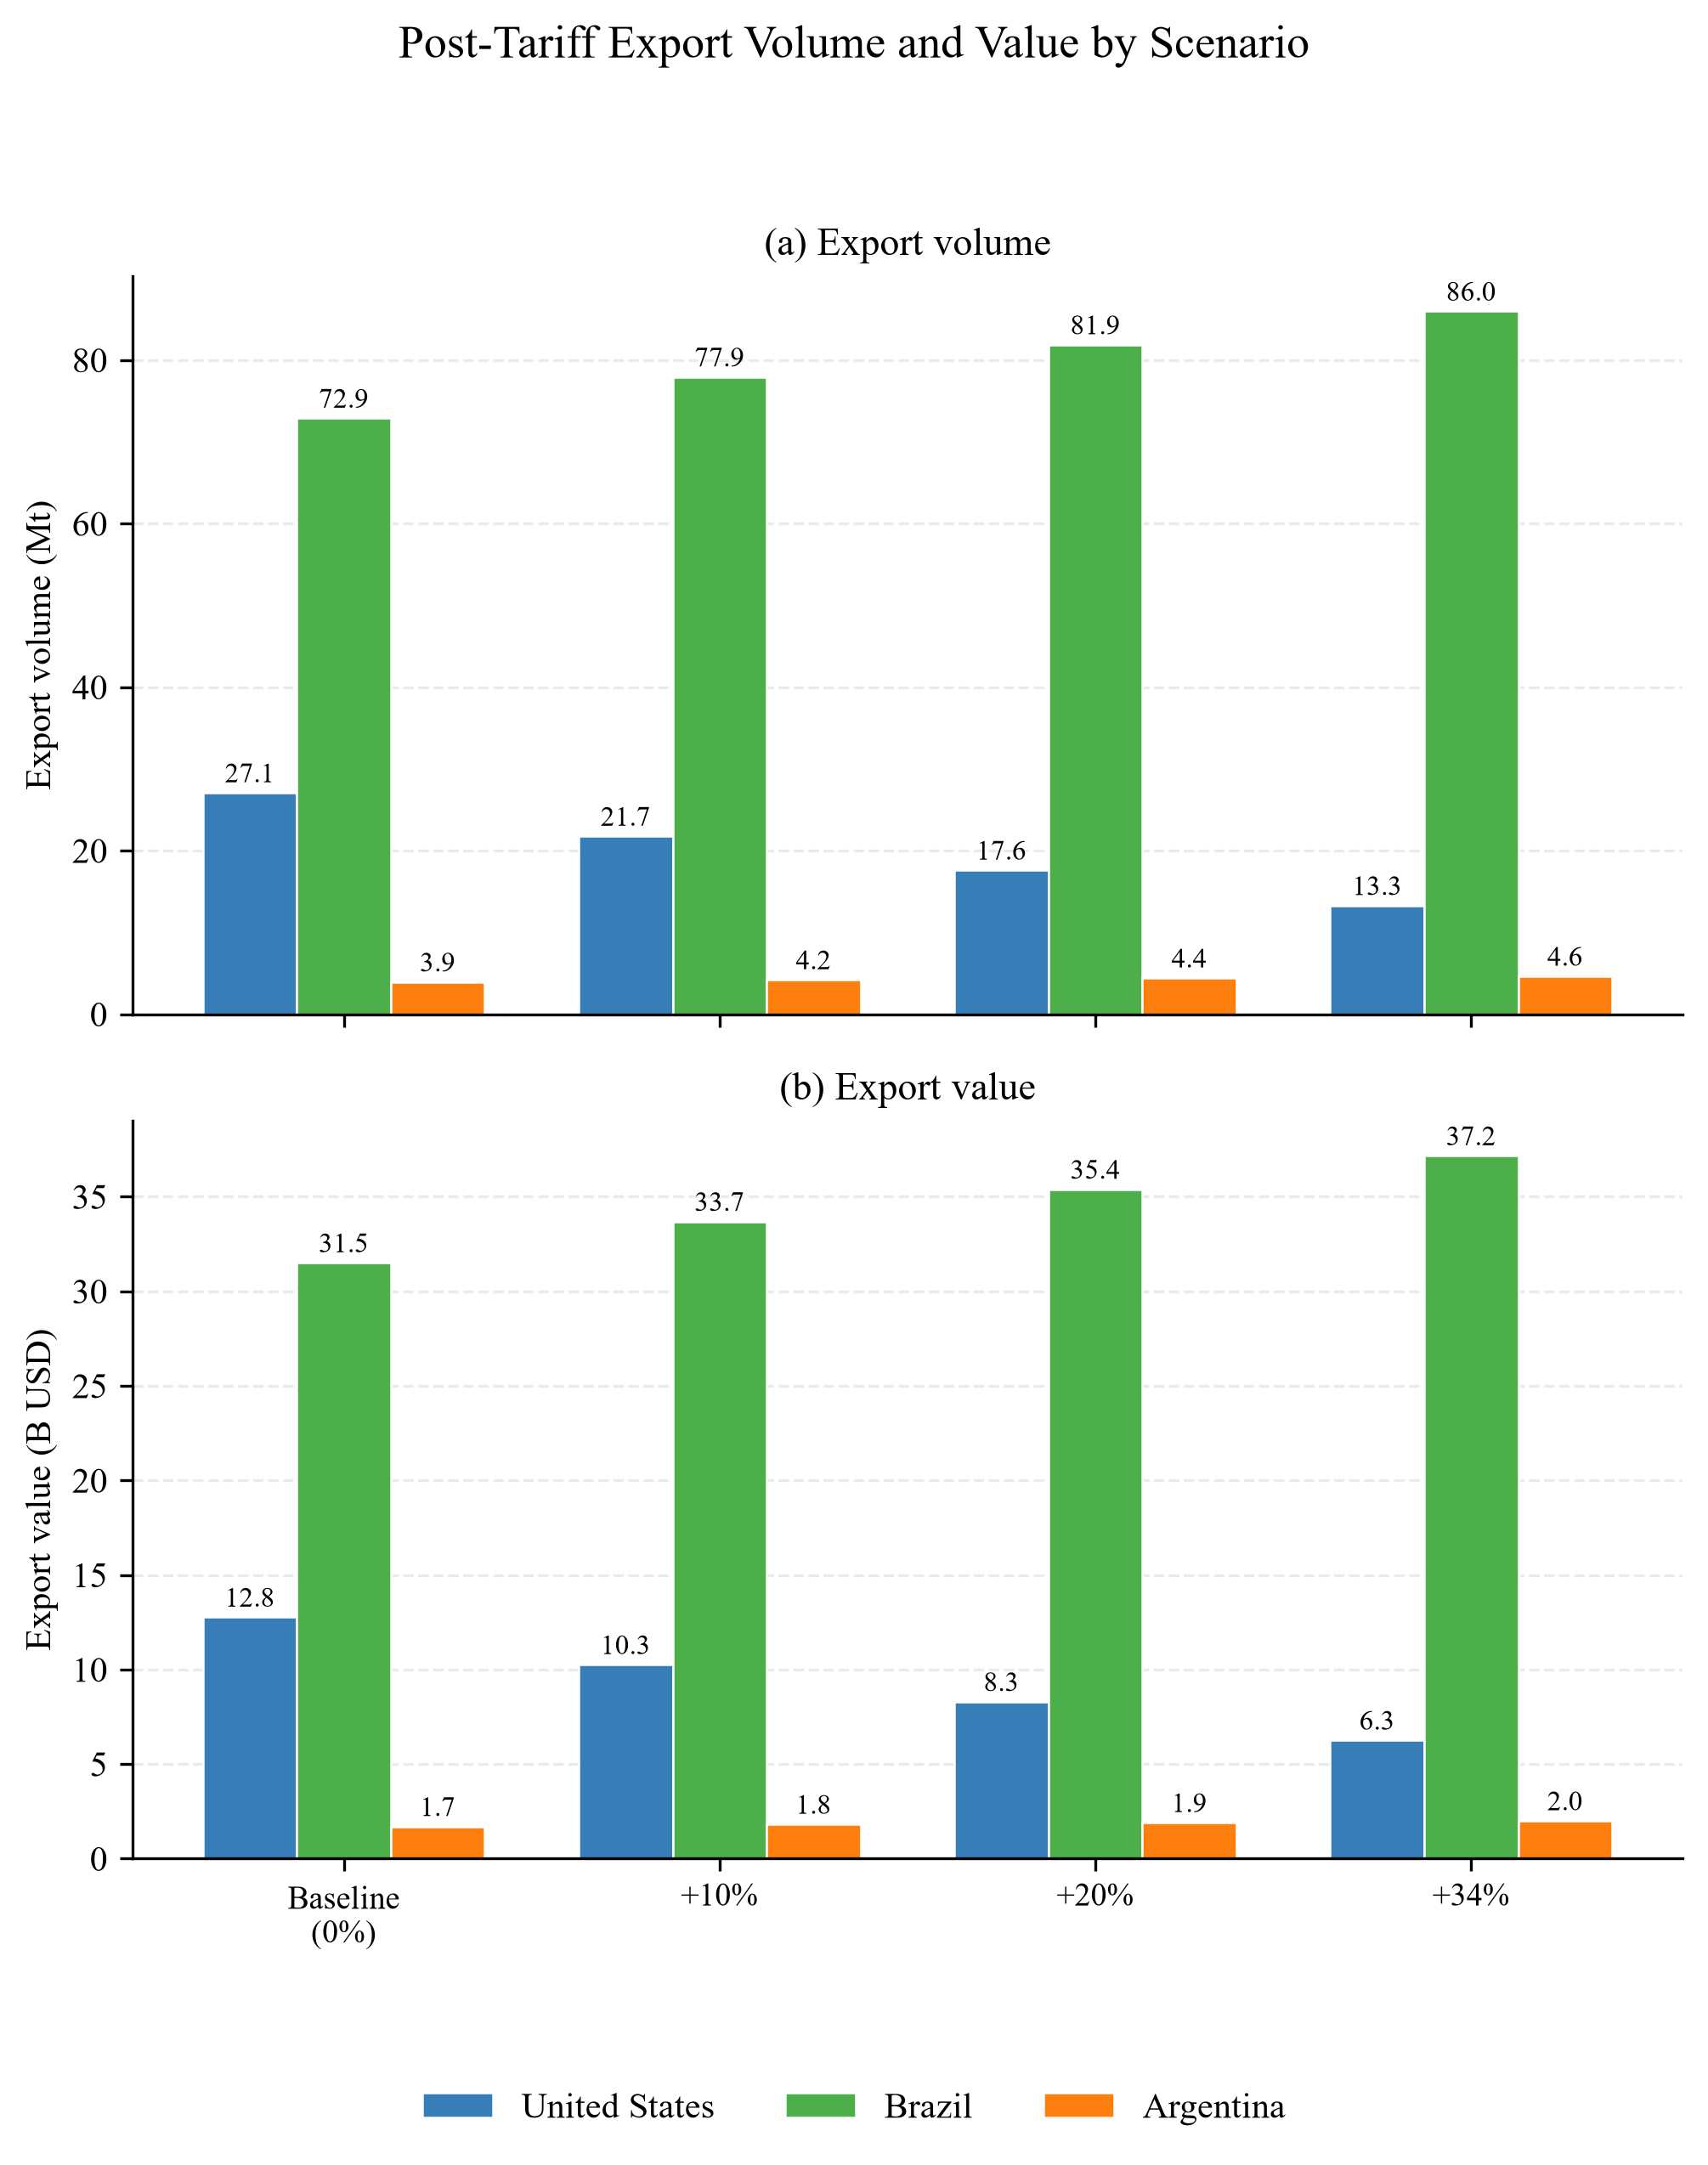
\includegraphics[width=0.9\textwidth]
    {../images/fig_scenario_qty_value.png}
    \caption{不同关税情景下中国大豆进口贸易的预测结果}
    \label{fig:scenario_qty_value}
\end{figure}

\begin{figure}[H]
    \centering
    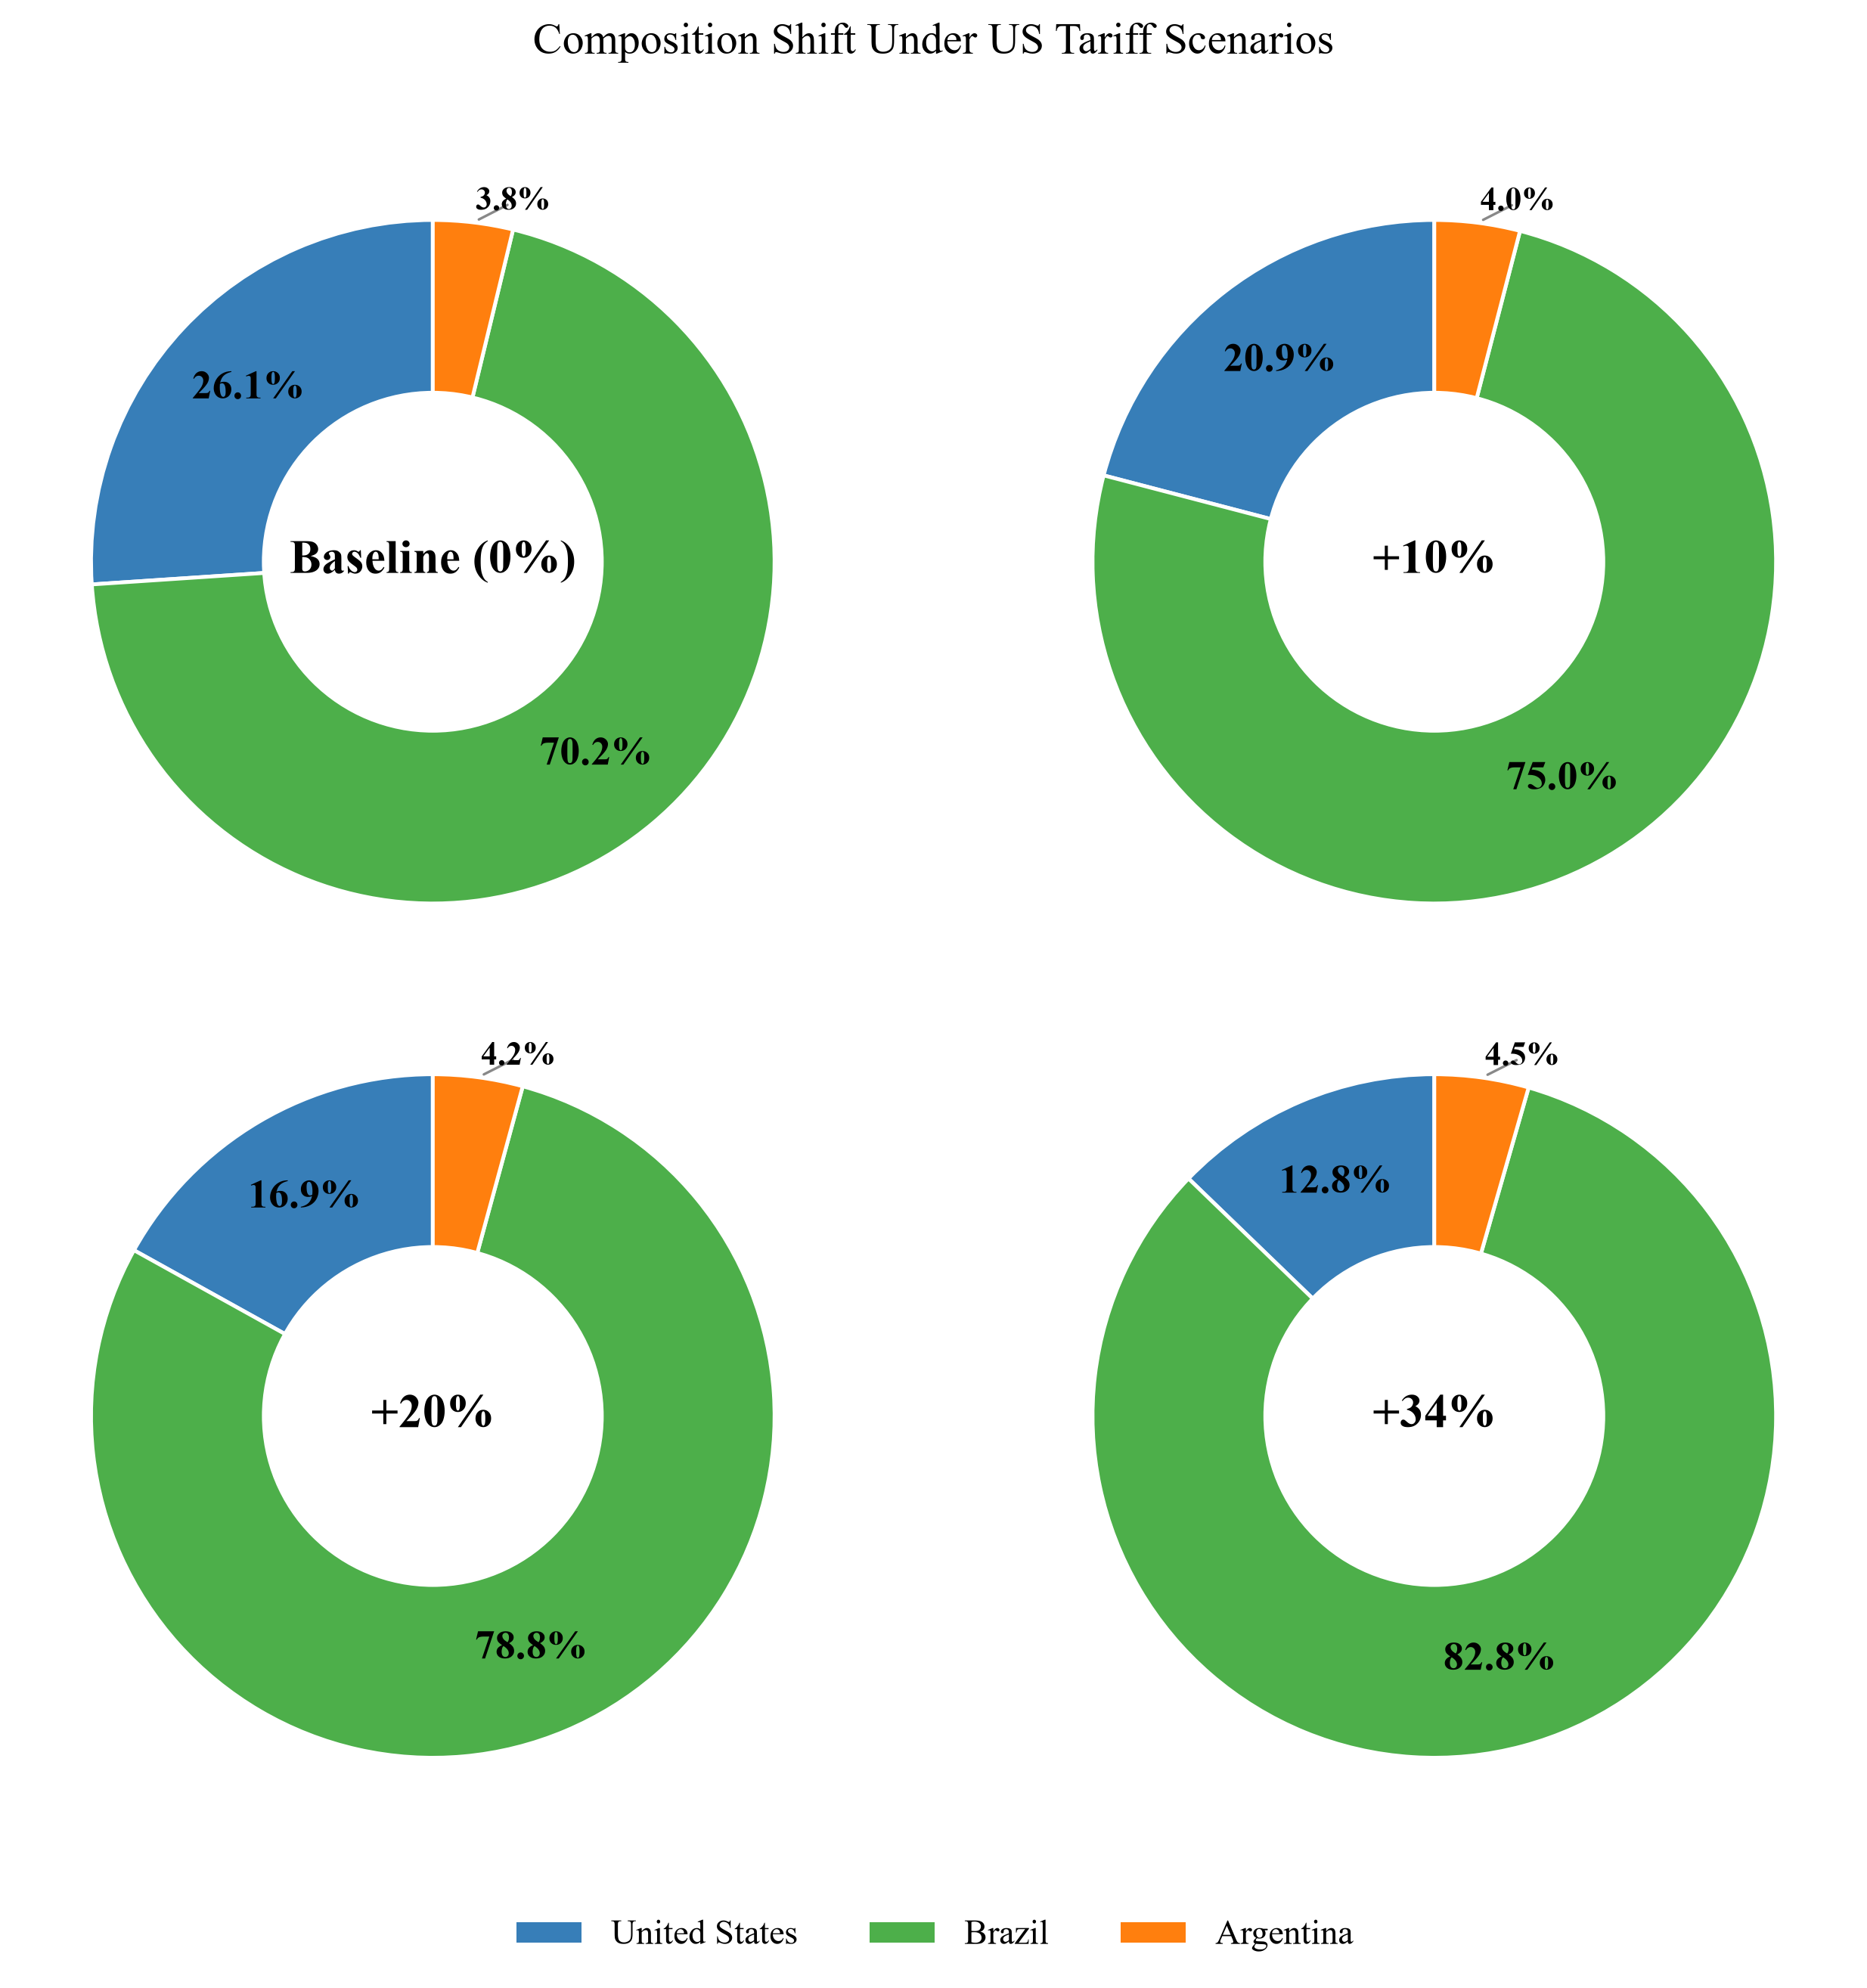
\includegraphics[width=0.75\textwidth]
    {../images/fig_scenario_donut.png}
    \caption{不同关税情景下中国大豆进口来源份额结构}
    \label{fig:scenario_donut}
\end{figure}

从不同关税情景下的预测结果可以看出，美国大豆的进口份额显著下降，而巴西和阿根廷的进口份额均呈上升趋势。其中，巴西进口份额的增幅高于阿根廷。为解释这一差异，本文进一步考察进口份额对基准价格变化的敏感程度，其偏导数可表示为：
$$
\frac{\partial s_i}{\partial P_i} = \frac{(1-\sigma)\alpha_i^\sigma P_i^{-\sigma}
\cdot \left( \sum_{j \neq i} \alpha_j^\sigma P_j^{1-\sigma} \right)}
{\left( \sum_j \alpha_j^\sigma P_j^{1-\sigma} \right)^2}
$$

根据模型假设，各出口国的基准出口价格保持不变，关税变化通过影响美国大豆的含税到岸价格，进而改变各国的进口份额。在此基础上，巴西和阿根廷的基准出口价格相近，但其来源国偏好参数 $\alpha_i$ 较大，因此，在相同关税变化所引起的相对价格调整下，巴西进口份额的增幅高于阿根廷。上述结果反映了基准价格与来源国偏好参数共同作用下，不同出口国进口份额对关税冲击的差异化响应。

\subsubsection{模型效果验证}

为检验所建立模型对关税政策变化及进口来源结构调整的解释能力，
本文选取2018年中美贸易摩擦期间的中国大豆进口贸易数据进行历史回测。

根据原始研究框架的设定，2018年中国对美国大豆加征的额外关税税率为25\%。
因此，本文以2017年作为基准年，利用2017年的实际贸易数据重新校准
来源国偏好参数$\alpha_i$，并将相应的关税冲击纳入模型，
预测2018年中国从美国、巴西和阿根廷进口大豆的份额。

为检验参数设定对预测结果的影响，
本文分别采用$\sigma=4.9$和$\sigma=4.0$两种替代弹性取值，
并进一步比较法定全额关税情景与半额关税对照情景下的预测表现。
相关预测结果与实际数据的比较如图~\ref{fig:verify_shares}所示。

\begin{figure}[H]
    \centering
    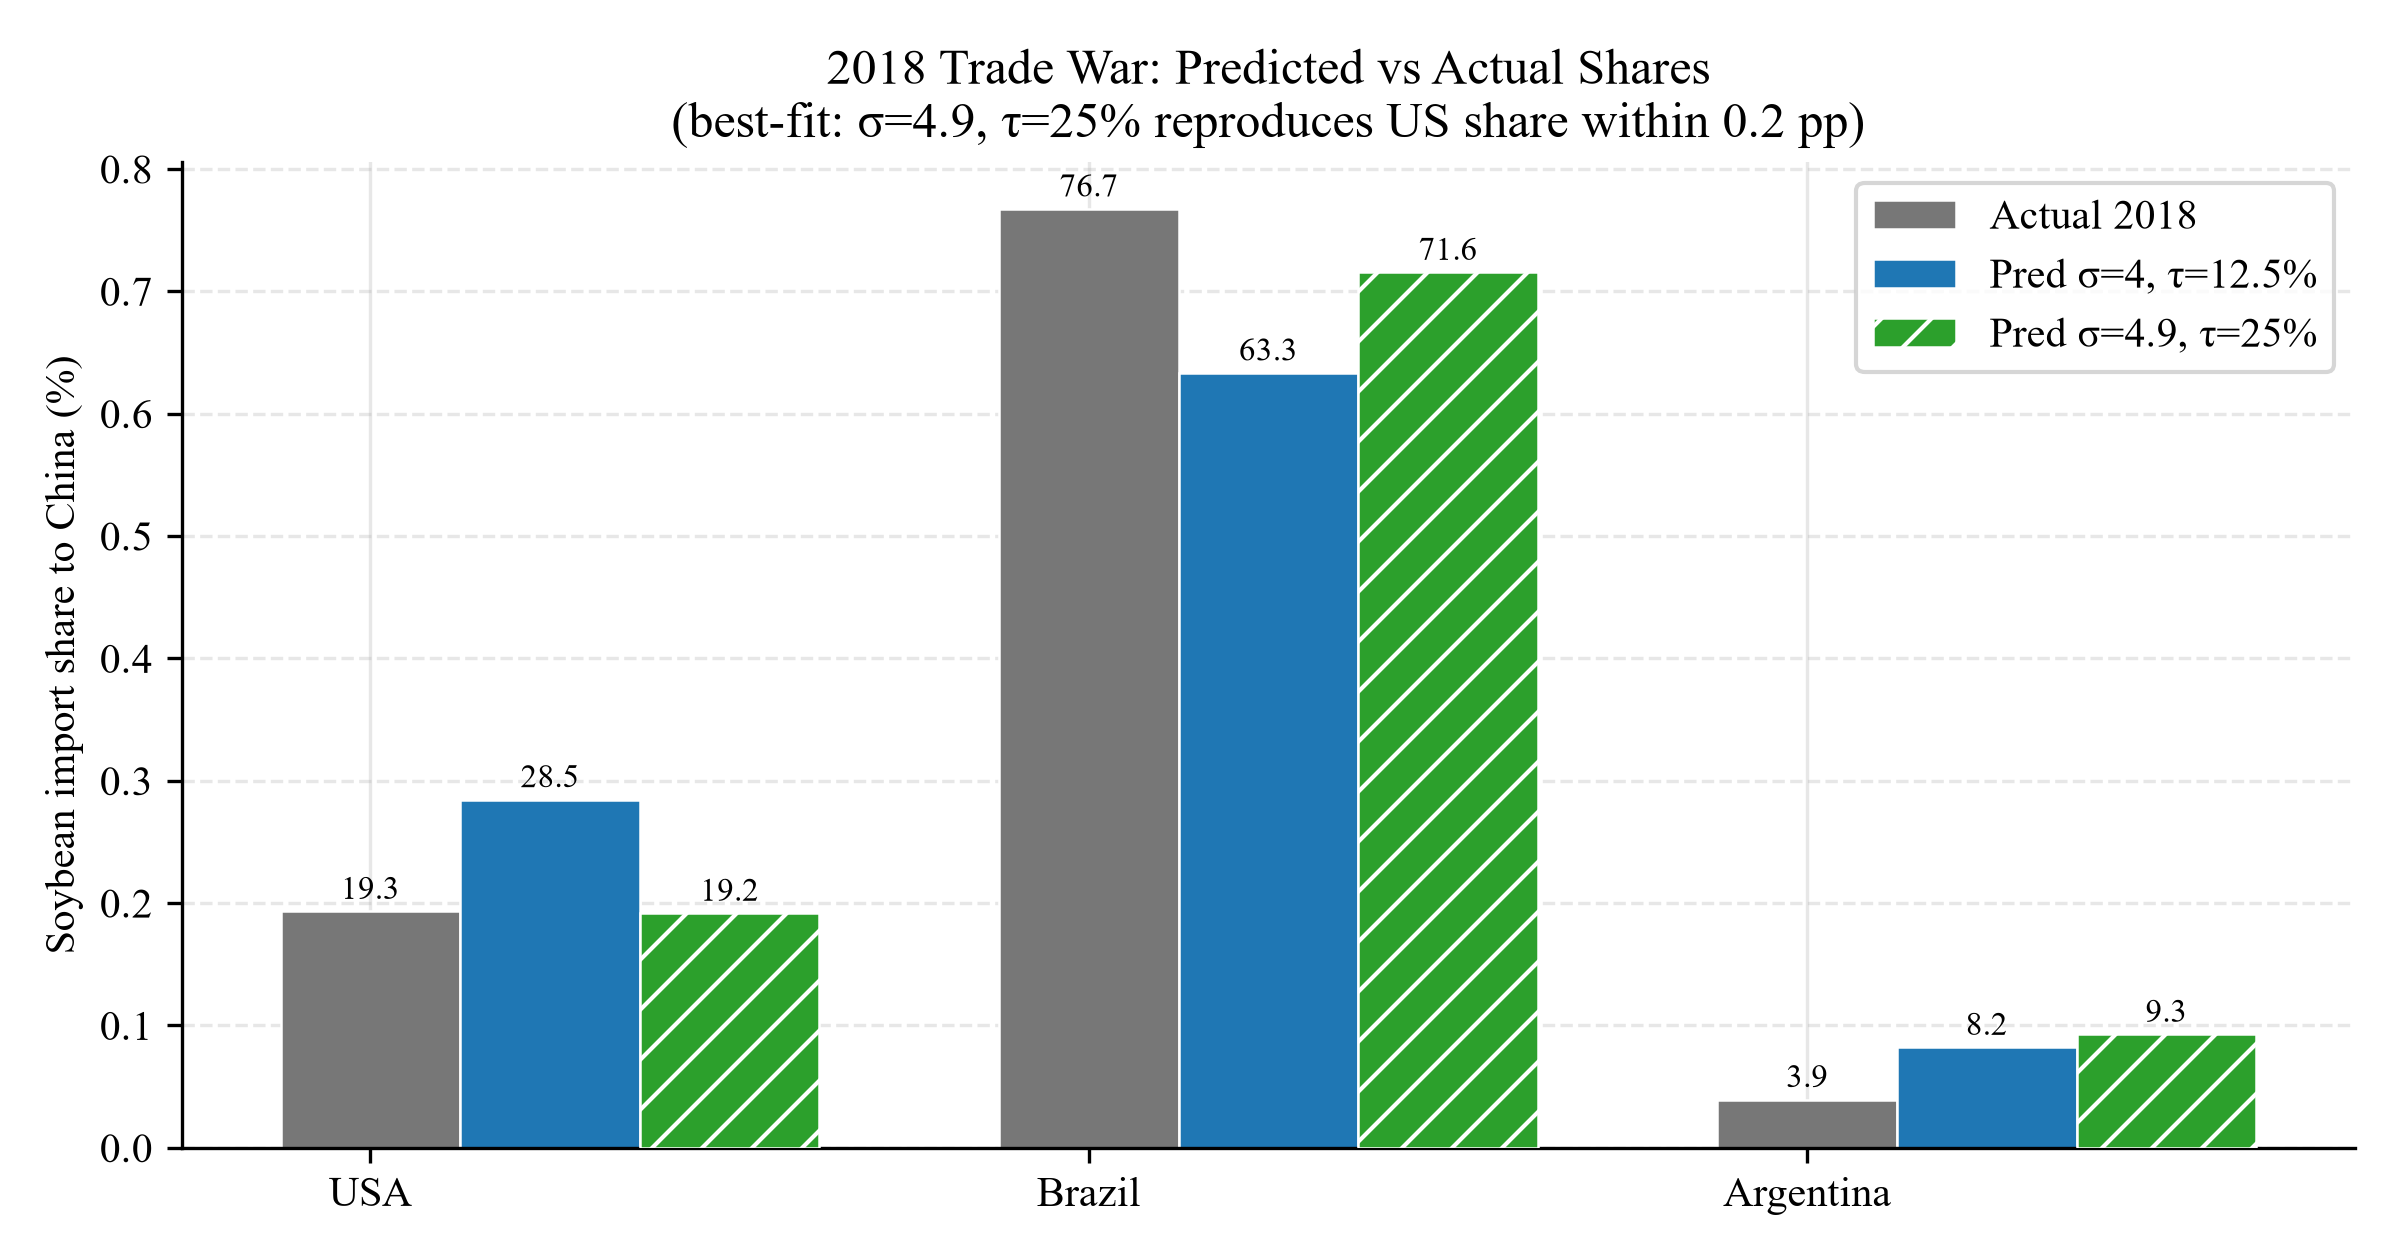
\includegraphics[width=1\textwidth]
    {../images/fig_verify_shares.png}
    \caption{2018年中国大豆进口来源份额的预测值与实际值比较}
    \label{fig:verify_shares}
\end{figure}

表~\ref{tab:verification_results}进一步列出了不同参数设定下
三国进口份额的预测值、实际值及平均绝对误差（MAE）。

\begin{table}[H]
    \centering
    \setlength{\tabcolsep}{4pt}          % 默认 6pt，调小
    \renewcommand{\arraystretch}{1.2}    % 行高
    \small
    \caption{2018年中国大豆进口来源份额的模型验证结果}
    \label{tab:verification_results}
    \begin{tabular}{lcccccccc}
        \toprule
        情景
        & $\sigma$
        & MAE \\
        \midrule
        $\tau=25\%$（法定全额，主）
        & 4.9
        & 0.036 \\

        $\tau=25\%$（法定全额）
        & 4.0
        & 0.054 \\

        $\tau=12.5\%$（半额关税，对照）
        & 4.9
        & 0.077 \\

        $\tau=12.5\%$（半额关税）
        & 4.0
        & 0.089 \\
        \bottomrule
    \end{tabular}
\end{table}

从表~\ref{tab:verification_results}可以看出，
在所比较的四组参数设定中，
$\sigma=4.9$且$\tau=25\%$的情景具有最低的MAE，
其美国大豆进口份额预测值为19.2\%，与实际值19.3\%较为接近。
相比之下，采用$\sigma=4.0$时，美国进口份额的预测值为22.5\%，
与实际值之间的差异有所增加。

对于巴西和阿根廷，模型预测结果与实际数据之间仍存在一定偏差。
在主情景下，巴西进口份额的预测值为71.6\%，低于实际值76.7\%；
阿根廷进口份额的预测值为9.3\%，高于实际值3.9\%。
这表明，模型虽然能够在一定程度上刻画关税冲击下的进口来源结构变化，
但其对不同国家进口份额的预测精度仍存在差异。

造成上述误差的潜在原因之一是，模型假设各国供给能力及其他非关税因素
在预测期间保持不变，而现实中的农产品贸易还会受到天气、产量、
出口供给及其他市场因素的影响。
例如，阿根廷在相关时期受到严重干旱影响，
其大豆生产和出口供给能力可能发生变化，
从而使实际出口份额偏离模型预测结果。

因此，预测值与实际值之间的差异可能部分反映了
供给冲击及其他未纳入模型的因素。
这一结果说明，在利用历史贸易数据检验模型时，
除关税政策外，还需要考虑各国生产能力和其他外部冲击的影响。
在现有假设下，本文模型可用于分析关税变化对进口来源结构的潜在影响，
但其预测结果仍需结合具体时期的实际贸易环境进行解释。

\section{Q2}

\subsection{this is a subsection of q2}
this is the content


%参考文献
\begin{thebibliography}{9}%宽度9
\bibitem{1} Author, Title, Place of Publication: Press, Year of publication.
\bibitem{2} author, paper name, magazine name, volume number: starting and ending
page number, year of publication.
\end{thebibliography}

\newpage
%附录

\section{Appendix}

\end{document} 